\chapter{Optimization in Locomotion}
\label{sec:OptimizationInLocomotion}
\index{optimization}

So far, this text has developed and analyzed various \textit{theoretical} models of locomotion without much attention to how animals actually choose to move around. What characterizes the way that animals naturally move around, and what factors influence this? Is locomotion mostly a passive mechanical behavior, or does it require subconscious cognition? How do our locomotion models compare to reality in the context of optimization? This chapter explores these question through some experiments that have been performed, and through the procedure of \textit{optimal control}. It is logical that animals are trying to optimize various quantities when choosing their motion, or when their mechanics choose their motion for them. It has long been hypothesized that animals move so as to minimize their energy use, a so-called ``principle of maximum laziness''. Such a principle was posited long ago, but is gradually being explored for various cases. Other factors though, such as joint wear, are also likely to play a role \cite{bertram01}. The knowledge of how and why animals choose a certain motion can be useful for physical training or other health-related issues, as well as for the design of energy-efficient robots.

[Things to add: Run motors fast to make them efficient., ]

\section{Energy Optimization Experiments} %(notes page 49-54)
\label{sec:EnergyOptimization}
\index{optimization}

This section focuses on two experiments that suggest animals exhibit a motion that minimizes the metabolic cost of the movement. The first experiment explores the natural relationship between the speed at which a human walks and how often the human takes a step. The second experiment explores how horses choose a gait (e.g. walk, trot, gallop).

\subsection{Speed-frequency relations}
\label{sec:SpeedFrequencyRelations}

The speed of a locomotive, for constant speed, is the distance traveled within a certain amount of time divided by that amount of time. If the locomotion is periodic, then the motion can be described with a step length $d$ and a step frequency $f$ (similar to wavelength and frequency for waves). Then, the speed of the periodic motion is

\begin{equation}
v = df
\label{eq:SpeedFrequency}
\end{equation}

Simple experiments performed in the 1980s posited that natural walking can be described by a correlation between speed and step frequency of the form

\begin{equation}
f = C v^{b} = Cd^{b/(1-b)}
\label{eq:StepFrequency}
\end{equation}

where $C$ and $b$ are empirical constants. As a result, if the speed $v$, step frequency $f$, or step length $d$ is known, the remaining two variables can be calculated from equations \ref{eq:SpeedFrequency} and \ref{eq:StepFrequency}. Human walking research has focused on the relations between $v$ and $f$ most likely because this data is easy to measure and analyze.

Now imagine an objective function $F$ that a locomotive naturally tries to minimize when moving around. This function $F$ could be the cost of transport, or it could be the amount of joint wear, or any other aspect of locomotion that may be desirable to minimize. Naturally, this function $F$ can depend on the entire description of the locomotion. $F$ most likely depends on the factors isometric srength and peak strain rate of muscles, the locomotive's weight, the locomotive's gait, joint angles, but certainly on speed, step length, and step frequency.

If the objective function $F$ is the cost of transport $COT$, it can be measured by the amount of $O_2$ consumed by a locomotive per unit distance it travels. A reasonable endeavor is to see how $F$ changes as only the factors of speed, step length, and step frequency are varied. We seek to find the minimum of the surface $F = F(v,f)$, where $d$ is given implicitly by equation \ref{eq:SpeedFrequency}. In this case, it is assumed that the surface $F$ has already been optimized for the other parameters such as joint angles. This surface is shown schematically in figure \ref{fig:Optimization} based on data from Molen \cite{molen72b} for the walking of male humans. The plot provides $O_{2}$ consumption per unit distance traveled as a function of $v$ and $d$, and implicitly $f$. Along a contour curve, the $COT$ is constant. If $F$ is well-defined (convex), it logically has a minimum for a certain pair of $v$ and $f$. This minimum is near the center of the contour curves.

% FIGURE
\begin{figure}[h]		% h="here" t="top" b="bottom" p="separate page"
\begin{centering}
\includegraphics[width=0.7\textwidth]{Figures/Optimization}\par
\end{centering}
\caption[Plot: Frequency-Speed and Oxgen Consumption Contours]{Frequency-speed and oxygen consumption contours. The curves A, B, and C come from experiment data points, and reveal a human' naturally chosen gait for fixed speed, fixed step frequency, and fixed step length, respectively. The contours show  oxygen consumption, a measure of the metabolic cost of transport, as a function of step frequency and speed. Figure is from \cite{needed} }
\label{fig:Optimization}
\end{figure}
%

Figure \ref{fig:Optimization} can help determine whether or not locomotives choose their motion so as to minimize energy cost. If this is the case, and if $F$ provides the energetic cost of transport, then the locomotive should choose \textit{naturally} the $v$ and $f$ that provide the minimum value of $F$ according to a plot like figure \ref{fig:Optimization}.

Furthermore, suppose the locomotive is constrained to move with either a fixed $v$, a fixed $f$, or a fixed $d$. Such a constraint is described by a straight line on figure \ref{fig:Optimization} that slices the surface $F$. A constrained $v$ is represented by a vertical line, constrained $f$ by a horizontal line, and constrained $d$ by a diagonal line emanating from the origin. In this constrained case, the locomotive should choose the motion that minimizes $F$ along that constraint line. This minimum value of $F$ must occur at a point where the contour curves of $F$ are tangent to the constraint line. This is the basis of the Langrage multiplier method of constrained optimization.

The three curves A, B and C in figure \ref{fig:Optimization} are constructed by connecting points at such minimum values of $F$ for a single given constraint line (e.g. $v = const.$), as the value of the constraint is varied (the constraint line is shifted). These three different constraint cases are explored in more detail.

\begin{itemize}
\item \textbf{Curve A, constant $v$}: Curve A is composed by connecting the points at the minimum of $F$ for a given fixed speed $v$, as the fixed speed $v$ is varied. An example of this case is a human walking on a treadmill that is set to a constant speed. The human chooses a step length or a step frequency, but must step at the speed of the treadmill in order to not fall off the treadmill. Based on the nature of the surface $F$ for human walking, curve A is slowly monotonically increasing.
\item \textbf{Curve B, constant $f$}: Curve B is composed by connecting the points at the the minimum of $F$ for a given fixed step frequency $f$, as the step frequency $f$ is varied. An example of this case is a human walking to the constant beat of a song. The human can still take small or large steps to control speed.  Based on the nature of $F$, curve B is monotonically increasing with a slightly steeper slope than curve A.
\item \textbf{Curve C, constant $d$}: Curve C is composed by connecting the points at the minimum of $F$ for a given step length $d$, as the fixed step length $d$ is varied. Again, on an $f-v$ plane constant step length is shown as a diagonal line going through the origin. The slope of this line is the value of $d$. An example of this case is a human that steps on only every fifth tile of a tiled floor. Based on the nature of $F$, curve C is monotonically decreasing.
\end{itemize}

These three constrained optimum curves A, B and C come directly from the shape of the contours. Also, the three curves all intersect at the minimum of $F$; this is a necessary feature of constrained optimization.

Imagine an experiment in which humans are asked to walk for a while as part of three different sets of walking trials. In the first set of trials, A, the human is instructed to walk at a given $v$, but to otherwise walk naturally. For each walking trial in this set, the human must walk at a different fixed $v$. The experimenter measures the step frequency $f$ that the human chooses. In the second set, $f$ is constrained and the chosen $v$ is measured. In the third set, $d$ is constrained and the chosen $v$ is measured. 

An empirical curve can be drawn on an $f-v$ plane for each set of trials. If the three empirical curves A, B and C are overlaid onto the constrained optimum curves A, B and C, all on an $f-v$ plane, and humans choose to naturally to walk so as to minimize $COT$, then empirical curve A should match constrained optimum curve A, and so on. This overlay would match natural walking data with energy minimization data. Thus, if the curves are the same, it means that natural walking is energy minimized walking. Of course, this experiment is much simpler than trying to develop an entire empirical surface $F$ (the entire surface $F$ is not actually required to develop any data used in the experiment).

Bertram, et al \cite{bertram01} performed the experiment described here, and found qualitative similarity between his empirical curves A, B and C, and the constrained optimum curves A, B and C, using data from Molen \cite{molen72b} to generate the constrained optimum curves. He found three mostly distinct curves A, B and C, with A and B monotonically increasing, B having a steeper slope than A, and C with either a small or negative slope. The experiment was performed on multiple humans, and the curves A, B and C varied between humans but the qualitative similarity did exist across humans. Additionally, all three curves intersected near the same point, hinting at an \emph{unconstrained} minimum point. Thus, his results buttress the hypothesis that humans naturally walk so as to minimize $COT$, even under constraints.

The experiments were actually conducted with a different aim in mind. Bertram, et al. sought to determine if equation \ref{eq:StepFrequency} holds true in general, or if it is only true for a subset of walking parameters. More precisely, does equation \ref{eq:StepFrequency} hold if the motion is constrained in some specific ways? A generally-applicable, and thus fundamental, equation would hold true regardless of the variation of other parameters. This means that empirical curves A, B and C would be exactly the same: the same step frequency is obtained for a chosen speed regardless of which parameter is held constant. Since Bertram, et al. found the three curves A, B and C to be distinct, he showed that equation \ref{eq:StepFrequency} is not as valid as was originially thought.

It is possible that the empirical curves are distinct from each other for reasons other than energy optimization. Perhaps a certain constraint causes the human to be more aware about certain aspects of his or her gait. If a human is required to walk with a fixed step length $d$ by being instructed to step on certain markings on a path, the human might focus his or her attention to the markers or ground more than he or she would if he or she was not constrained.

\begin{comment}
old notes:
-Ruina has done these experiments and found similar shapes. [HINTS]
The similarity between experimental results and the $F = COT$ surface.
-Then say: Ruina has explored this experimentally: has found qualitatively similar shapes, intersection of 3 curves nearly at the same point. See paper for experimental results.
Equation \ref{eq:SpeedFrequency} does not capture the full nature of walking, as it does not hold for all possible sets of constraints
-Conducted an experiment that indicates that humans, when walking, minimize the cost of energy given the constraints imposed on the motion.
Experiment: 3 distinct speed-frequency curves depending on the constraint
Assumption that walking person minimizes $F(v,f)$: 3 distinct speed-frquency curves 
-An experiment done by Molen \cite{molen72b} provide $O_{2}$ consumption contours qualitatively similar to those in figure \ref{fig:Optimization}.
-Ruina originially sought to see if the f = Cvb law was fundamental.

\cite{bertram01}

Molen \cite{molen72b}

to still include:
- COT surface varies depending on individual.
- of course, in Ruina's experiments it is not known for sure that the humans were choosing to walk as a result of external factors related to the type of constraint imposed. Pehraps one constraint is more natural than another.

\end{comment}

\subsection{Choosing a gait}
\label{sec:ChoosingAGait}

\begin{comment}
-introduce gaits
-analogy to gears
-at least humans and horses optimize energy with choice of gait
-cost as a function of speed: no extended gaits; get one curve
-cost as a function of speed: with extended gaits, start to see some variation, curvilinear
-cost per speed as function of speed: -if the data for each gait is edited, we see minima
-histogram: unforced, 
-two things to explore: cost per gait, for extended gaits

discovery: within each gait, there is an optimum energy usage

farley A mechanical trigger for the trot-gallop transition in horses 

MINETTI METAPHOR: BIOMECHANICS AND BIOLOGY OF MOVEMENT. , CHANGING GAITS IS LIKE CHANGING GEARS ON A BIKE \cite{nigg00}
Any model of locomotion must be associated with a particular \textit{gait}\index{gait}. 

TALK ABOUT WHY MEASURING OXYGEN IS SUFFICIENT; CHEMICAL VS MECHANICAL ENERGY. TALK ABOUT WHY MEASURING OXYGEN IS SUFFICIENT. TALK ABOUT WHY MEASURING OXYGEN IS SUFFICIENT. TALK ABOUT WHY MEASURING OXYGEN IS SUFFICIENT
\cite{hoyt81}

1-NEED ARTICLE ABOUT HUMANS
2-finish outline, considering extended gaits issue
\end{comment}

We have seen evidence that humans optimize their motion according to $COT$ when walking, but this case is only one case out of all of the possible locomotion scenarios. It concerns only one species and considers only walking. Can we make similar statements about energy optimzation for other animals, and if the motion is not confined to walking? In this section, we explore energy optimization for the motion of horses that are walking, trotting, or galloping.

A walk, a trot, and a gallop are all gaits\index{gait}. A gait is a certain periodic movement of legs \cite{hildebrand89}. Examples of human gaits are walking and running. When walking, there is a period of time when both legs contact the ground. When running, only one foot is ever in contact with the ground, and the contact accounts for a smaller portion of the motion. A gait can be characterized with a gait diagram. This type of diagram indicates the duration of time that each foot or leg of an animal is in contact with the ground. Of course, a gait can have characteristics that are not capured by such a diagram, such as the motion of the legs while they are not in contact with the ground.

In a horse's walking gait, each of the four legs is in contact with the ground for about 70\% of the gait cycle. About every quarter of a gait cycle, the horse puts down the next of four legs. In the trotting gait, the horse alternates between placing pairs of opposing legs (e.g. front left and rear right) on the ground. Each pair of legs is in contact with the ground for roughly 50\% of the gait cycle. In a gallop, the rear horse alternates between the rear pair and front pair of the legs, and each pair contacts the ground for only about 25\% of the gait cycle. This means that for a substantial portion of the gait, neither pair of legs makes contact with the ground.

What factors affect how a locomotive chooses a gait? This question was explored experimentally by Hoyt \cite{hoyt81} for the case of horses, and can be answered by a series of assertions.

\textbf{Ignoring gaits, the relation for horses between metabolic cost of transport and speed is linear.} In this experiment, a horse is required to move at a certain speed without any regard to gaits. This is easily enforced by placing the horse on a treadmill. The metabolic cost of transport is measured by the rate of oxygen consumption. Between speeds of 1 m/s and 6 m/s, a horse's rate of oxygen consumption is a linear function. At the speed of 6 m/s, a horse's rate of oxygen consumption is about 100 mL O$_2$/s.

\textbf{If a horse is constrained to use a certain gait, the metabolic cost of transport is no longer a linear function of speed.} Under the previous assertion, the horse chooses its own gait based on the speed it must travel. A horse can be trained to extend its gaits. That is, the horse uses a gait at speeds at which it would typically use a different gait. This allows the generation of three curves for metabolic cost, one for each gait, as a function of speed. These three curves approximate the curve from the previous assertion, but curve upwards at the speeds where the gait is extended. As a result of this curvature, the three concave-up curves intersect at the points where a horse would change gaits. This is required for the three curves to approximate a line if extended gaits are dropped from the plot. This means that for any speed the metabolic cost of operating in an extended gait is always higher than the metabolic cost of operating in the natural gait.

% FIGURE
\begin{figure}[h]		% h="here" t="top" b="bottom" p="separate page"
\begin{centering}
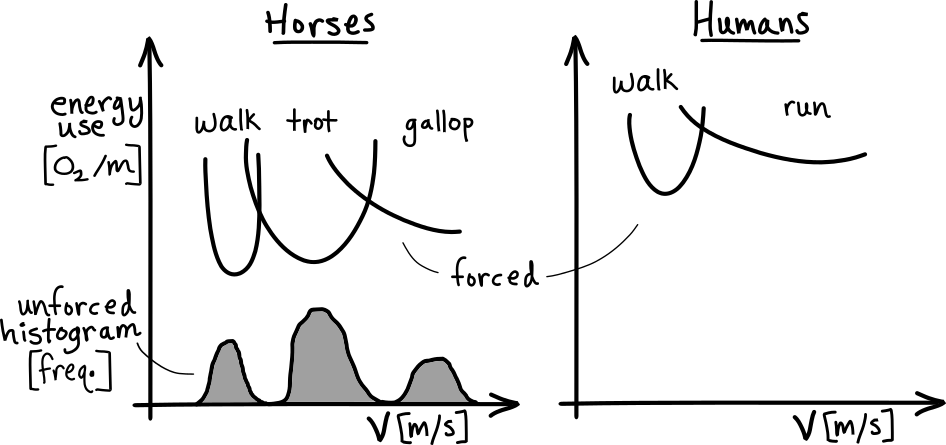
\includegraphics[width=0.8\textwidth]{Figures/HorseLocomotion}\par
\end{centering}
\caption[Plot: Energy Use vs Speed for Horses and Humans]{Energy use vs speed for horses and humans. The oxygen consumed per meter traveled, ``energy use'', is shown across three horse gaits. Horses and humans choose the gait that requires the least oxygen consumption per meter traveled. Within each gait, there is a minium value for ``energy use'', and this minimum occurs at roughly the same value for all gaits for horses.}
\label{fig:HorseLocomotion}
\end{figure}
%

\textbf{For each gait, there exists a speed at which the energy to move a unit distance is at a minimum.}  The energy to move a unit distance is given by dividing speed into the metabolic cost. If the related quantity, volume O$_2$ consumed to move 1 meter, is plotted against speed, the three curves from the previous assertion are transformed into the steep curves in the left plot of figure \ref{fig:HorseLocomotion}. Logically the walking gait is used for the slowest speeds, the trot is used for the middle speeds, and the gallop is used for the fast speeds. The portion of the walking curve that extends into the trotting region comes from an extended walking gait, and it is evident that a walking gait at trotting speeds requires more energy than trotting at those speeds.

Additionally, it is clear that for each gait, there is a minimum energy to move a unit distance. Interestingly, this minimum occurs around the same value for each gait. That means each gait has the same energy cost if a horse travels at the speed that is energetically optimal for that gait. This nature of the locomotion supports an analogy that locomotives choose gaits much like a bikerider uses gears on a bike \cite{nigg00}. A bikerider chooses gears that makes sense, in terms of energy effiency, for a certain speed. Thus when using gears, it is possible for a bikerider to use the same energy cost to travel 1 meter when travelling at 3 m/s as when travelling at 6 m/s.

\textbf{Horses naturally choose to move at the energetically optimal speed for a given gait.} This assertion is the key that connects what has been asserted about the existence of an optimum energy for each gait, and how horses choose a gait naturally. The shaded curve in figure \ref{fig:HorseLocomotion} is a histogram describing the number of times a horse travels at the corresponding speed on the horizontal axis. There are clear peaks at the speeds corresponding to optimized energy for each gait, showing that a horse naturally chooses to move at an optimal speed.

The same effect observed here for choosing gaits with horses can also be observed for humans. However the optimal energy cost for 1 meter of travel is greater than for horses. However, this optimal value is again largely independent of gait.

[talk more about humans?]

% FIGURE
\begin{figure}[h]		% h="here" t="top" b="bottom" p="separate page"
\begin{centering}
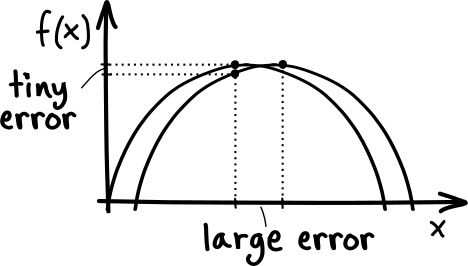
\includegraphics[width=0.4\textwidth]{Figures/BadPredictor}\par
\end{centering}
\caption[Diagram: Optimization is a Bad Predictor]{Optimization is a bad predictor. When trying to deduce input parameters that produce optimal output characteristics, working backwards in an optimization can produce large errors. The diagram shows an arbitrary function that has shifted in the x-direction. If one is looking at the output value $f(x)$ and trying to find the corresponding x, the shift will produce only a very small error in $f(x)$, yet the shift in x that caused the error could be quite large.}
\label{fig:BadPredictor}
\end{figure}
%

\section{Optimal Control} %(notes page 50-60, 64)
\label{sec:OptimalControl}
\index{control!optimal}

The experimental work presented in section \ref{sec:EnergyOptimization} seems to show that legged animals choose gaits and locomotive behaviors that minimize energy use. Though they are not proof, the individual cases strongly indicate that energy use is an important factor in determining the way animals walk, run, and trot. Could this have been predicted with a model?

Predicting this behavior requires both a model of locomotion and a way of somehow optimizing the model's gait. It is easy to see that this is an optimization problem because there is one scalar parameter to be minimized: energy use. What is less clear is what must be changed about the model's gait to find the point at which energy use is minimal. It turns out that this parameter to be changed is actually a function of time. 

% FIGURE
\begin{figure}[h]		% h="here" t="top" b="bottom" p="separate page"
\begin{centering}
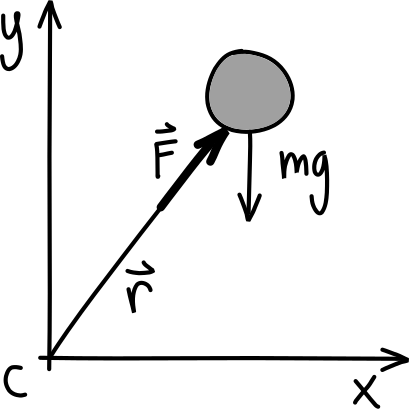
\includegraphics[width=0.25\textwidth]{Figures/PointMass}\par
\end{centering}
\caption[Diagram: A Point Mass in 2D Space]{A point mass in two-dimensional space. This figure is often the starting point for the simplest model of locomotion.}
\label{fig:PointMass}
\end{figure}
%

Start with the simplest model of locomotion: the point mass model. Figure \ref{fig:PointMass} shows the point mass with a force acting on it. Imagine that the force acting on the point mass can vary with time, and its direction points in the same direction as the vector $\vr$. The vector $\vr$ stretches from point C to the point mass, where point C is the location of an imagined foot touching the ground. The foot does not move, allowing the point mass to rotate about point C, if the leg connecting the foot and point mass were rigid. Here, the length of the leg can vary. The motion of the point mass is determined by the linear momentum balance shown in equation \ref{eq:PointMassLMB}:

\begin{equation}
F(t)\frac{\vr}{|\vr|}-mg\hat{j}=m\va
\label{eq:PointMassLMB}
\end{equation}

From this momentum balance, we can extrapolate the velocity of the point mass in the x-direction and the rate of change of the distance between point C and the point mass. With these two rates, we can find a value for the energetic cost of transport, or $COT$. The $COT$ is the value that we are trying to minimize. In chapter \ref{sec:Introduction}, the idea of the $COT$ was introduced as:

\begin{equation*}
\mbox{cost of transport}=\frac{\mbox{positive muscle work}}{\mbox{weight}*\mbox{distance}} 
\end{equation*}

In this particular case, the $COT$ becomes the following:

\begin{equation}
COT=\frac{\int_{0}^{T}[F(t)\dot{l}(t)]^{+}dt}{mg*\int_{0}^{T}V_{x}dt}
\label{eq:PoinMassCOT}
\end{equation}

Here, $\dot{l}(t)$ is the rate of change of the distance between point C and the point mass. This quantity times the force as a function of time, $F(t)$, is the power function $P(t) = F(t)\dot{l}(t)$. However, it is assumed that the leg is only doing work when it is pushing off of the ground, so the power function is taken as zero if $P(t) \leq 0$. This is noted by square brackets and a plus symbol, which say:

\begin{align}
[\mbox{...}]^{+} &= [\mbox{...}] \mbox{ if } [\mbox{...}] > 0 \notag \\
&= 0 \mbox{ if } [\mbox{...}] \leq 0 \notag
\label{eq:PowerBracketNotation}
\end{align}

For this problem, a constraint on the motion of the point mass requires that $F(t)$ satisfies $V_{y}(T) = 0$, where $T$ is the half-time for a step. Before setting this up as an optimization problem, consider what a force function of time, $F(t)$ might look like. Figure \ref{fig:ForceOptimization} shows two possible force functions for two different gaits, over a the half-time $T$ of a gait. The solid line represents approximately what walking looks like, while the dotted line approximates running. These force functions can be generated experimentally by using a simple force plate measurement system like the one in figure \ref{fig:ForcePlate}. 

% FIGURE
\begin{figure}[h]		% h="here" t="top" b="bottom" p="separate page"
\begin{centering}
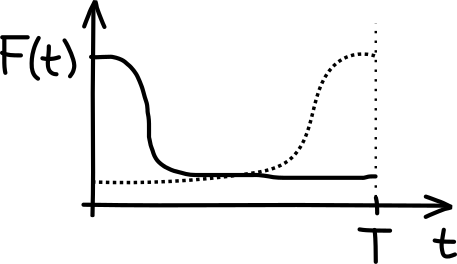
\includegraphics[width=0.4\textwidth]{Figures/ForceOptimization}\par
\end{centering}
\caption[Plot: Optimal Force Profiles for Bipedal Locomotion]{Optimal force profiles for bipedal locomotion. The solid line represents approximately what walking looks like, while the dotted line approximates running. These force functions can be generated experimentally by using a simple force plate measurement system like the one in figure \ref{fig:ForcePlate}. }
\label{fig:ForceOptimization}
\end{figure}
%

To discover a force function $F(t)$ in time that minimizes the $COT$, some kind of iterative optimization package must be used. The sheer magnitude of possible solutions to the optimization problem requires computer help. A good program for solving this problem is SNOPT \index{SNOPT} for MATLAB, but before working with such an optimization package, it is good to first have an understanding of optimal control in general. A short guide to solving optimal control problems with SNOPT can be found in appendix \ref{sec:UsingSNOPT}.

The central piece of optimal control is the objective function. The objective function is a function is a function of many parameters $F_{obj}(x_{1}, x_{2}, ... x_{n})$ that a program like SNOPT tries to make as big or as small possible by modifying the input parameters in a systematic way. The objective function is a scalar function.

%%______________________________________________________________
%%
%% ALAN: Things I don't fully understand, but that were mentioned in class: the Simplex Method, linearity/non-linearity of the objective function, and the objective function as an equality vs inequality. 
%%_____________________________________________________________

The next piece of optimal control are the constraint functions. There can be one or many constraint functions that bound the problem and tell the optimizing package where to look. For example, figure \ref{fig:ObjectiveFunction} shows a general objective function and two constraint functions. Imagine that the objective function is a bowl of sorts, and the goal is to reach the bottom of the bowl, shown here as the smallest circle. The circles represent level lines of the objective function, so it makes sense that the smallest circle of the level lines could be either a peak or a valley. The constraint functions are then where the optimizer looks for the solution. The constraints could be such that the two lines define an area on which the optimizer can search, or they could be such that the optimizer is limited to solutions that lay directly on the lines themselves. For this example, in the latter case, the constraints would prevent the optimizer from finding the true minimum of of the objective function. In general, a constraint function would look something like $G(x_{1},x_{2}) = N$, where the parameters $x_{n}$ of $F_{obj}$ and $G$ are the same parameters, and $N$ is a constant defined by the problem at hand. 

% FIGURE
\begin{figure}[h]		% h="here" t="top" b="bottom" p="separate page"
\begin{centering}
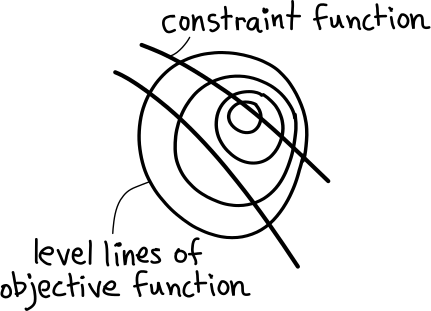
\includegraphics[width=0.4\textwidth]{Figures/ObjectiveFunction}\par
\end{centering}
\caption[Diagram: Objective Functions and Constraint Functions]{Two constraint functions on an objective function. The level lines of the objective function represent a three-dimensional surface. The constraint functions constrain the results of optimization problem further by removing one of the three dimensions of the objective function or establishing a relationship between two of the variables.}
\label{fig:ObjectiveFunction}
\end{figure}
%

In the case of optimal control, the goal is not simply parameter optimization, rather the goal is to find some control function in time that minimizes energy use; the optimizer attempts to minimize $F_{obj}(F(t))$, where $F(t)$ is some input function of time. In the world of legged locomotion, $F(t)$ is a ``coordination pattern" or ``control function." The function $F_{obj}$ is also called a ``functional" since it takes a function in time as an input and outputs a scalar value. 

%%______________________________________________________________
%%
%% Side note: Hamilton's Principle: poses $\vF=m*\va$ as an optimization problem, spurring modern physics. 
%%______________________________________________________________

There are a few different methods for solving optimal control problems. One could use calculus of variations, or one could use dynamic programming, a generalization of calculus of variations that utilizes the Pontriagan maximization principle. Alternatively, one could reduce the problem to parameter optimization by approximating the function $F(t)$ with parameters $x_{1}, x_{2}, ... x_{n}$. There are many ways to do this, for example with a Fourier series or a Taylor series. However, a piecewise constant function lends itself well to programming in MATLAB with optimization programs such as SNOPT. Figure \ref{fig:PiecewiseConstant} shows what an arbitrary function looks like approximated as a piecewise constant function. Each ``step'' in the function becomes a parameter, where the precision of the optimization program can be tuned by specifying the number of parameters to use to approximate the function. 

% FIGURE
\begin{figure}[h]		% h="here" t="top" b="bottom" p="separate page"
\begin{centering}
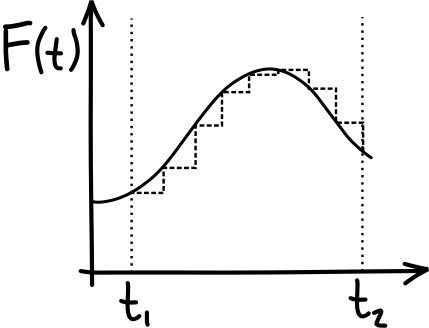
\includegraphics[width=0.35\textwidth]{Figures/PiecewiseConstant}\par
\end{centering}
\caption[Plot: Piecewise Constant Approximation of Input Function]{Piecewise constant approximation of an input function of time. This discretization simplifies the optimization problem such that the problem is tractable. The more pieces the user defines, the longer it takes for the solver to find the correct input function. As indicated in the plot, the user must also specify bounds on the horizontal axis, or in this case, the time boundaries of the input function.}
\label{fig:PiecewiseConstant}
\end{figure}
%

Remember that our goal is to find the ``best" control function, $F(t)$. The objective function $F_{obj}(x_{0}, x_{1}, \mbox{...}, x_{n})$ is the $COT$ from equation \ref{eq:PoinMassCOT}. Remember also that the power function $P(t)=F(t)\dot{l}(t)$ is only valid when positive, which is noted by the square brackets $[\mbox{...}]^{+}$. However, this function $[P(t)]^{+}$ presents a problem because it is not smooth at the origin, and therefore causes a non-smoothness in $F_{obj}$ that is problematic for optimization packages like SNOPT \index{SNOPT}. Consider figure \ref{fig:SmoothedFunction}, which shows the function $[P(t)]^{+}$ as a function of $P(t)$. To be able to use $[P(t)]^{+}$ in the objective function, a smoothed version of the function must be created.


% FIGURE
\begin{figure}[h]		% h="here" t="top" b="bottom" p="separate page"
\begin{centering}
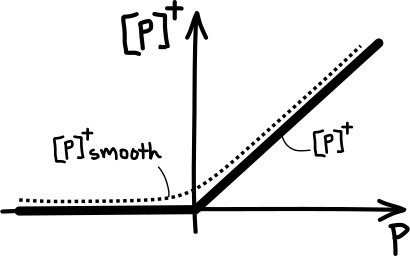
\includegraphics[width=0.4\textwidth]{Figures/SmoothedFunction}\par
\end{centering}
\caption[Plot: Smooth Power Function]{Smoothing the power function. To use the power function $P=F(t)\dot{l}(t)$, it must be multiplied by a function (solid line) that will make the power function only exist when positive. The unit-ramp function can accomplish this for us. However, because of the non-smooth point at the origin, the unit-ramp function causes problems for the optimization solver. The function must be smoothed for it to work with the optimization solver (dotted line).}
\label{fig:SmoothedFunction}
\end{figure}
%

To smooth the power function $[P(t)]^{+}$, a little trick is used. While it is difficult to come up with a smooth version of $[P(t)]^{+}$ as shown in figure \ref{fig:SmoothedFunction}, it's easier to come up with a smooth version of its derivative. After creating a smooth version of the derivative of $[P(t)]^{+}$, integrating that function will yield a smooth version of $[P(t)]^{+}$. The derivative of $[P(t)]^{+}$ is a step function, shown in figure \ref{fig:IntegralFunction}.

% FIGURE
\begin{figure}[h]		% h="here" t="top" b="bottom" p="separate page"
\begin{centering}
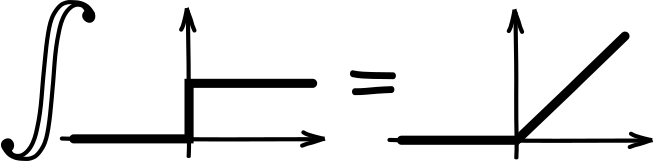
\includegraphics[width=0.4\textwidth]{Figures/IntegralFunction}\par
\end{centering}
\caption[Diagram: Creating an Integral Function]{The unit-ramp function is difficult to describe mathematically as a smooth continuous function of the input variable, so we use a simple trick: find a mathematical description for the unit-step function, and integrate. The integral of the unit step function is the unit-ramp function, so we will get a reasonably accurate mathematical description of the unit-ramp function that is continuous and smooth.}
\label{fig:IntegralFunction}
\end{figure}
%

To approximate a step function as a smooth function, we can use the logistic function, shown in figure \ref{fig:LogisticFunction}.

% FIGURE
\begin{figure}[h]		% h="here" t="top" b="bottom" p="separate page"
\begin{centering}
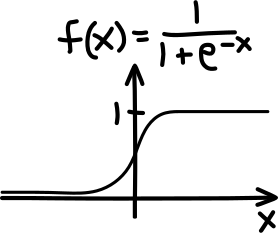
\includegraphics[width=0.18\textwidth]{Figures/LogisticFunction}\par
\end{centering}
\caption[Plot: the Logistic Function]{The logistic function. The logistic function can be used to describe the unit-step function if the correct tuning parameter is applied, as in equation \ref{eq:LogisticFunctionTuned}. By tuning the logistic function, we can get it to look more like the unit-step function, which can then be integrated to get a mathematical description of a smooth continuous unit-ramp function.}
\label{fig:LogisticFunction}
\end{figure}
%

But notice that the top and bottom of the logistic function are not sharp right angles like in the step function. To create a sharper logistic function, a tuning parameter $\epsilon$ must be added to the function, where $\epsilon$ is an infinitely small number. The tuned logistic function then becomes:

\begin{equation}
f(x)= \frac{1}{1+e^{-x/\epsilon}}
\label{eq:LogisticFunctionTuned}
\end{equation}

Finally, integrating equation \ref{eq:LogisticFunctionTuned} gives a function that we can use to approximate the ramp function $[P(t)]^{+}$:

\begin{equation}
\int f(x) = \epsilon ln(e^{x/\epsilon}+1)
\label{eq:IntegralFunctionTuned}
\end{equation}

In both equation \ref{eq:LogisticFunctionTuned} and equation \ref{eq:IntegralFunctionTuned}, the variable $x$ should be replaced with the entire function $P(t)$ to get $[P(t)]^{+}$ as the end result. The smoothed positive function $[P(t)]^{+}$ can then be used in the objective function $F_{obj}$ and solved with an optimizer like SNOPT. Roughly, SNOPT is a Sequential Quadratic Program (SQP). Where gradient-based methods take the derivative of a function, sequential quadratic methods take the second derivative of a function. SNOPT tries to find the minimum of the function approximated as a quadratic. \index{SNOPT}
